\section{HPC software, relevant qualities and software engineering methods}

\textit{High performance computing} (HPC) is the platform technology concerned with programming for performance (speed), energy efficiency (doing more with less power), upscaling (handling larger problems), or high throughput (handle large volumes of data in near real-time).

\subsection{Parallel and distributed computing}

Several years ago, HPC and \textit{parallel and distributed computing} (PDC) were regarded as the same thing. Nowadays, they are distinct (but overlapping.

\begin{figure}[H]
	\centering
	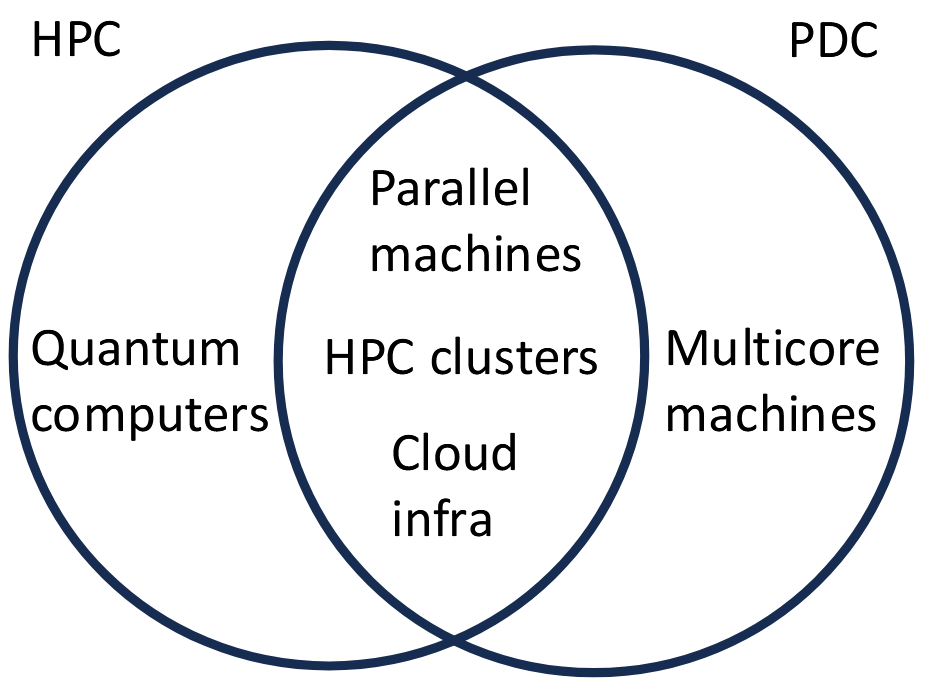
\includegraphics[width=0.3\linewidth]{images/hpc-vs-pdc}
\end{figure}

The main characteristics of PDC are \textit{concurrency} (more than one active execution context), \textit{parallelism} (execution of different tasks at the same time), and \textit{distribution} (execution of different tasks on physically different interconnected computing nodes, without a global clock). The following image shows the differences between distributed and parallel computing.

\begin{figure}[H]
	\centering
	\begin{minipage}[t]{0.27\linewidth}
		\vspace{0pt}
		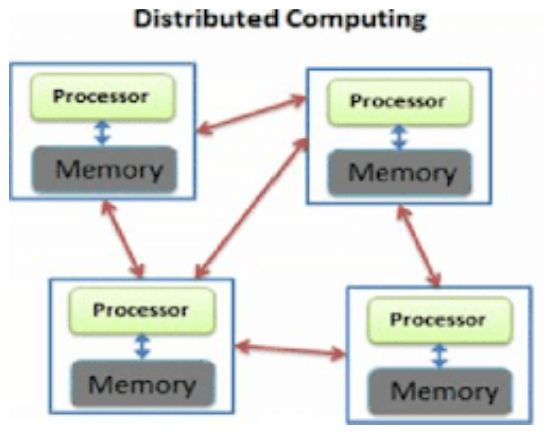
\includegraphics[width=\linewidth]{images/distributed-computing}
	\end{minipage}%
	\hspace{0.05\linewidth}%
	\begin{minipage}[t]{0.25\linewidth}
		\vspace{0pt}
		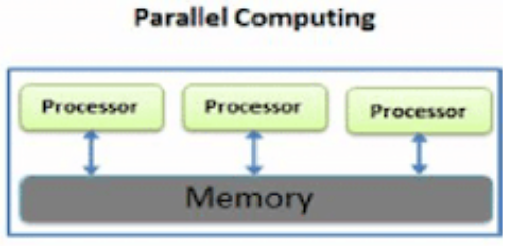
\includegraphics[width=\linewidth]{images/parallel-computing}
	\end{minipage}
\end{figure}

\subsection{Qualities of HPC software}

HPC applications can be subdivided in two categories:

\begin{enumerate}
	\item \textbf{Compute-intensive applications}. Concern complex computations requiring a large number of computational resources. They often require parallel computing. Compute-intensive software must ensure: \textit{correctness}, \textit{performance}, \textit{portability}, \textit{maintainability}.
	\item \textbf{Data-intensive applications}. Focus on processing, storing and retrieving large amounts of data. They are typically built as distributed systems to ensure reliability and scalability. Data-intensive software must ensure: \textit{reliability}, \textit{scalability}, \textit{maintainability}.
\end{enumerate}
